\section{Model and Experiments}

%This section is a mix of models and experiments. This is the main section of the report which will log the entire research process. You will write down the precise description of the model, experiment design, results, graphs, analysis of results, next set of experiments, and so on.
%
%As the model evolves over time, do not edit the already described model. Write a new version of the model. Treat this section as a research log. Not as a research paper.
%
%Use the images folder to put all your images. Use \textit{meetings.tex} to maintain a log of all the project meetings and weekly to-do list.

\subsection{Neural network version of BrownBuild}

The BrownBuild initiative classifies failed builds as being brown (unreliable) or safe (true failures). This binary classification is based on a XGBoost classifier. 
To be able to apply Continual learning approaches, the first step is transform the classification model into a Neural Network (NN): in fact, NN can be used in online learning, so that updates can be done while the model is used instead of retraining from scratch when a modification in needed.

\Do{add parameters tested}

\Do{add final results for this part}

\subsection{Continual learning with a NN model for BrownBuild detection}

We know have to define a Continual Learning set-up for the project. 


\begin{figure}[h]
    \centering
    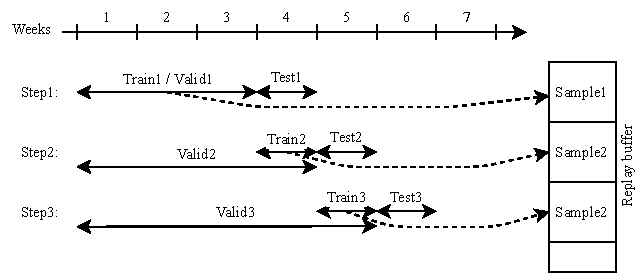
\includegraphics{img/CLUbi_sets.pdf}
    \caption{Set-up of the different sets during the Continual Learning process.}
    \label{fig:CL_set_setup }
\end{figure}
% This need to be compared to the results of concept drift that was computed in the BrownBuild paper (ADD REF). 

